%% by Michael Shell
%% Edited by Rohan Sikder
%%
%% This work is distributed under the LaTeX Project Public License (LPPL)
%% ( http://www.latex-project.org/ ) version 1.3, and may be freely used,
%% distributed and modified. A copy of the LPPL, version 1.3, is included
%% in the base LaTeX documentation of all distributions of LaTeX released
%% 2003/12/01 or later.
%% Retain all contribution notices and credits.

\documentclass[11pt,journal,compsoc]{IEEEtran}

\hyphenation{op-tical net-works semi-conduc-tor}

\usepackage{lipsum} 
\usepackage{hyperref}
\usepackage{biblatex}
\usepackage{graphicx}
\usepackage{listings}

\graphicspath{{images/}}

\addbibresource{test.bib}

\begin{document}
% paper title
% Titles are generally capitalized except for words such as a, an, and, as,
% at, but, by, for, in, nor, of, on, or, the, to and up, which are usually
% not capitalized unless they are the first or last word of the title.
% Linebreaks \\ can be used within to get better formatting as desired.
% Do not put math or special symbols in the title.
\title{Object Detection: \\ Innovations and Real-World Applications}

% author name
\author{Rohan~Sikder% <-this % stops a space
}

% The paper headers
\markboth{Research Methods in Computing \& IT - Literature Review}%
{}

\IEEEtitleabstractindextext{
    \begin{abstract}
        This particular literature review explores the considerable developments in object detection technology. With a main focus on the newest advancements in YOLOv8 and the practical applications of its. Object detection is an important part in different fields such as automotive safety, healthcare, and surveillance, and has developed immensely with the launch of neural networks and deep learning. Original methods including simple feature and template matching detection, made way for more complicated techniques as deep learning and machine learning triggering breakthroughs just like the convolutional neural network (CNN) and YOLO architecture. YOLOv8 has proven great advancements over the predecessors of its in terminology of efficiency, accuracy, and speed, which makes it an invaluable tool in real time object detection applications. This particular evaluation dives into the evolution of object detection strategies, from beginning techniques on the YOLOv8, analyzing the algorithmic improvements of its accuracy enhancements and pragmatic implications. Additionally, it addresses the problems and limitations of current investigation, especially in ethical concerns and complex environments surrounding privacy. The review concludes by showcasing the demand for future investigation, especially in the improvement of specialized hardware such as FPGAs and also in the exploration of ethical dimensions of object detection.
    \end{abstract}
}

% make the title area
\maketitle

\section{Introduction}
\label{sec:introduction}
\IEEEPARstart{T}{he} field of object detection technology has made significant improvements, particularly with computer vision. This technology is vital in various applications, from surveillance systems to self-driving cars. This review of the literature aims to explore the growth and current state of object detection technologies, emphasizing the latest developments in YOLOv8 and its practical implications.


\subsection{Overview of Object Detection Technology:}
The ability to detect and find objects in photos and videos is a significant technological achievement in computer vision. Applications ranging from surveillance systems to self-driving cars depend on this. The YOLO architecture (you only look once) is one of the many object detection methods that have been created. YOLOv8 has made improvements that solve problems and extend what is possible of real-time object identification.
\subsection{Advancements in Object Detection, Practical Applications and Benefits:}
This literature review looks deeply into object detection, particularly into advancements and research. First, Presenting a review of the development of object detection techniques, highlighting the improvements made by the YOLOv8 architecture, such as region-based Convolutional Neural Network (R-CNN), Single Shot Detector (SSD), and YOLOv8. Secondly to describe how these developments can actually benefit practical applications in areas like automotive safety, healthcare, security, and surveillance where accuracy and speed have to be regularly balanced.

\subsection{Objective and Scope:}
This will be done by reviewing studies and publications.This review is to address the challenges that have been solved and those that continue within object detection. It also explores how YOLOv8 and its features and capabilities, contributes to resolving some of the issues in object detection, such as reducing false positives and improving detection in complex environments. This review aims to identify the gaps in current research. Inclusion criteria for this review include studies and publications that focus on advancements in object detection algorithms, such related to the YOLO series, and it's practical applications in different application's. Exclusion criteria studies and publications that are primarily theoretical and have no practical application in object detection, or those that do not contribute directly to the understanding or improvement of the YOLO architecture and its implementations.

\section{Evolution of Object Detection Techniques}
\subsection{Early Techniques and Limitations:}
 Early simple techniques like template matching, such as comparing small parts of an image (template) with a larger image, to find matches and simple feature detection, such as edges or corners, which were limited in their complexity and efficiency. An early object detection algorithm was the Viola-Jones algorithm, in particular, face detection. However, it was limited to frontal faces only and struggled with various poses and lighting.\cite{990517}


\subsection{Breakthroughs in Object Detection}
Object Detection has seen significant advancement with the introduction of machine learning and deep learning. 
\subsubsection{Machine Learning}
Support Vector Machines (SVM's) a machine learning algorithm are used for object detection which improved accuracy over traditional methods. This still depended on manually selected features to help the algorithm read images. A study found that using a Support Vector Machine (SVM) classifier with a faster R-CNN system for analyzing retinal images in medical settings led to better results. This decreased the rate of incorrect identifications (false positives) by about 30\% but slightly increased the rate of missed detection's (false negatives) by around 16\% \cite{kurilova2021support}. The SVM was quite accurate, correctly classifying images around 85\% of the time on average and in the best case up to 92\%\cite{kurilova2021support}. This shows that combining SVM with faster R-CNN can improve the accuracy of detecting specific features in medical images.
\subsubsection{Deep Learning Revolution}
The emergence of convolutional neural networks (CNN's) created a great leap in object detection. AlexNet, a deep CNN, won the ImageNet challenge by a large margin in 2012 for demonstrating the use of deep learning power in object recognition. The network achieved an error rate of 15.3\%, which was more than 10.8\% points lower than that of the runner up\cite{wiki:alexnet}. CNN works by processing data that have a grid-like topology, such as images, through a series of layers that automatically and adaptively learn spatial hierarchies of features. Deep learning enabled object recognition in complex and dynamic environments, real-time processing, and greater accuracy across diverse contexts that were previously not possible with traditional methods.

\begin{figure}[ht]
  \centering
  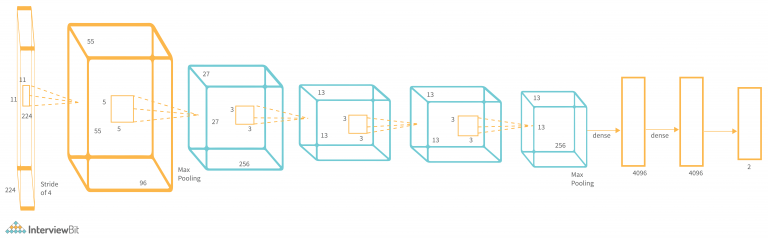
\includegraphics[width=0.5\textwidth]{images/cnn_architecture.png} 
  \caption{Architecture of a convolutional neural network.}
  \label{fig:cnn}
\end{figure}

\subsection{From R-CNN to SSD: Progression}
Progression is seen from Regions with Convolutional Neural Networks (R-CNN) to Single Shot MultiBox Detector (SSD) significantly.  R-CNN, a concept introduced by Ross Girshick et al, used something called Region Proposals. This means the R-CNN system scans through an image and suggest various 'regions' or specific areas where it suspects objects might be. These suggestions are similar to an initial guess of where important stuff could be in a picture.

Once these regions are created. R-CNN uses a Convolutional Neural Network (CNN) to closely check each proposed area. It is like taking a magnifying glass and looking closely at each guess to understand what is actually there. This detailed look helps to find the characteristics or 'features' of the objects in these regions. To make sense of these features and decide whether the object is a cat, a dog, or a car. R-CNN uses a type of region classifier known as an SVM, which stands for Support Vector Machine.\cite{Girshick_2014_CVPR} Think of SVM as a complex decision-making tool that, after looking at all the features provided by CNN, makes a final decision on what the object is.

SSD\cite{9262816} significantly simplified this process. Instead of taking the time to propose regions and then analyze them, SSD divides the image into a grid from the start. As it scans the image, it instantly identifies and categorizes objects within each grid cell. This approach is much more efficient because it combines the steps of proposing regions and classifying them into one process. Like quickly scanning a crowd and recognizing faces , which makes SSD much better for applications where quick processing is required, such as in real-time video analysis.

\begin{figure}[ht]
  \centering
  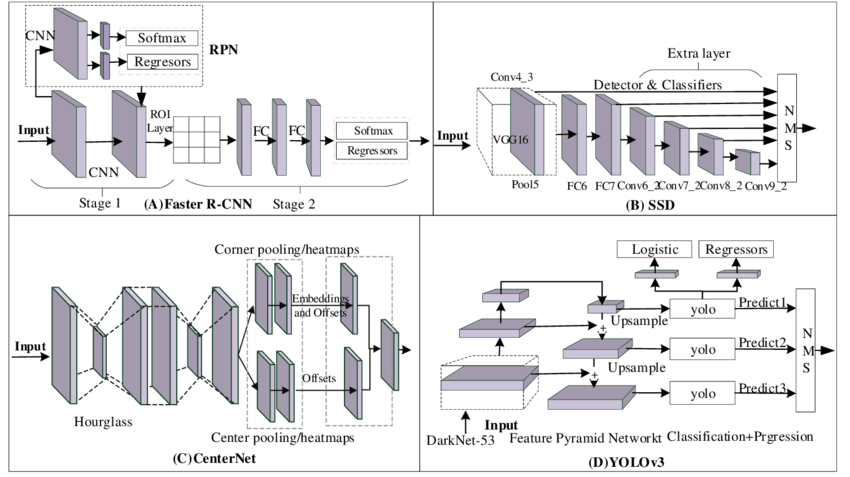
\includegraphics[width=0.5\textwidth]{images/progression_comparison.png} 
  \caption{Comparative architectures of object detection techniques including (A) Faster R-CNN, (B) SSD, (C) CenterNet, and (D) YOLOv3.}
  \label{fig:progression comparison}
\end{figure}



\section{The YOLO Architecture: Overview}
YOLO (You Only Look Once) is a very popular object detection and segmentation model, it was developed by Joseph Redmon and Ali Farhadi in University of Washington and launched in 2015. YOLO is a popular model for several reasons. It is fast, accurate, easy to use, and open-source. It has also been cited more than 42,000 times in academic papers\cite{Redmon_2016_CVPR} and has thousands of forks and stars on the YOLO repository on GitHub\cite{ultralytics}. Since then, YOLO has reached its eighth iteration YOLOv8.\cite{yolov8_ultralytics}

\subsection{Basics of YOLO (You Only Look Once)}
The architecture is unique from traditional methods of object detection, as it processes detection in a single pass from conventional generating region proposals and then classifies objects within the region proposal. This single operation significantly reduces computational power and allows real-time object detection applications.\cite{yolov8_ultralytics}

\subsubsection{YOLO's approach to object detection}
YOLO relies on dividing the image into a grid of cells. For each cell, the model predicts multiple bounding boxes, each representing a potential object. Along with these bounding boxes, YOLO also predicts the object's class probability, indicating the likelihood of the object being one of the recognized categories\cite{Redmon_2016_CVPR}.

In the latest version of YOLO, YOLOv8 has introduced features and improvements for improved performance and efficiency. Now it fully supports vision AI tasks such as detection, tracking, and classifications.YOLOv8 uses pre-trained Detect models, and the main one they use is the COCO data set.\cite{ultralytics2023models}

\subsection{Accuracy and Speed Enhancements}
YOLOv8 is seen in detection of fractures in pediatric wrist trauma X-ray images using data augmentation. This addresses a need in hospital emergency departments where paediatric wrist trauma fractures are a common and challenging issue , With the use of YOLOv8  in this context has shown its performance.

From studying learning data augmentation strategies for object detection \cite{zoph2020learning}, data augmentation is described as a process of artificially expanding the training data set for machine learning models. This is done by creating variations of existing data. This is done by altering the images in different ways, as would happen in real-world cases. Rotating, scaling, cropping, or adjusting the lighting and colour of images is commonly done. These techniques help the model learn to recognize objects or patterns in different contexts this leads to improved generalizing and performs accurately on new data.

By using data augmentation techniques, YOLOv8 really improved performance and accuracy. The YOLOv8 model got a mean average precision (mAP) of 0.638 on the pediatric wrist trauma X-ray data set (GRAZPEDWRI-DX) \cite{ju2023fracture}, outperforming both the improved YOLOv7 and the original YOLOv8 models. This accuracy is crucial in medical settings where precise diagnosis is critical.

\begin{table}[ht]
\centering
\caption{Evaluation of wrist fracture detection with other state-of-the-art (SOTA) models on the GRAZPEDWRI-DX dataset. Reproduced  from \cite{ju2023fracture}.}
\label{tab:wrist_fracture_detection}
\begin{tabular}{lcccc}
\hline
\textbf{Model} & \textbf{Precision} & \textbf{Recall} & \textbf{F1} & \textbf{mAP\textsubscript{val} 50} \\
\hline
YOLOv5\textsubscript{53} & 0.682 & 0.581 & 0.607 & 0.626 \\
YOLOv7\textsubscript{32} & 0.556 & 0.582 & 0.569 & 0.628 \\
YOLOv7\textsubscript{32} + CBAM\textsubscript{70} & 0.709 & 0.593 & 0.646 & 0.633 \\
YOLOv7\textsubscript{32} + GAM\textsubscript{71} & 0.745 & 0.574 & 0.646 & 0.634 \\
YOLOv8\textsubscript{36} & 0.694 & 0.679 & 0.623 & 0.636 \\
Ours & 0.734 & 0.592 & 0.635 & 0.638 \\
\hline
\end{tabular}
\end{table}



The development of "Fracture Detection Using YOLOv8 App"\cite{ju2023fracture} directly shows YOLOv8's practicality. Which helps pediatric surgeons in reading X-ray images. This reduces the probability of errors in fracture diagnosis and provides valuable information for surgeries. This application shows the potential of YOLOv8 to help medical diagnostics and improve patient care.

\begin{figure}[ht]
  \centering
  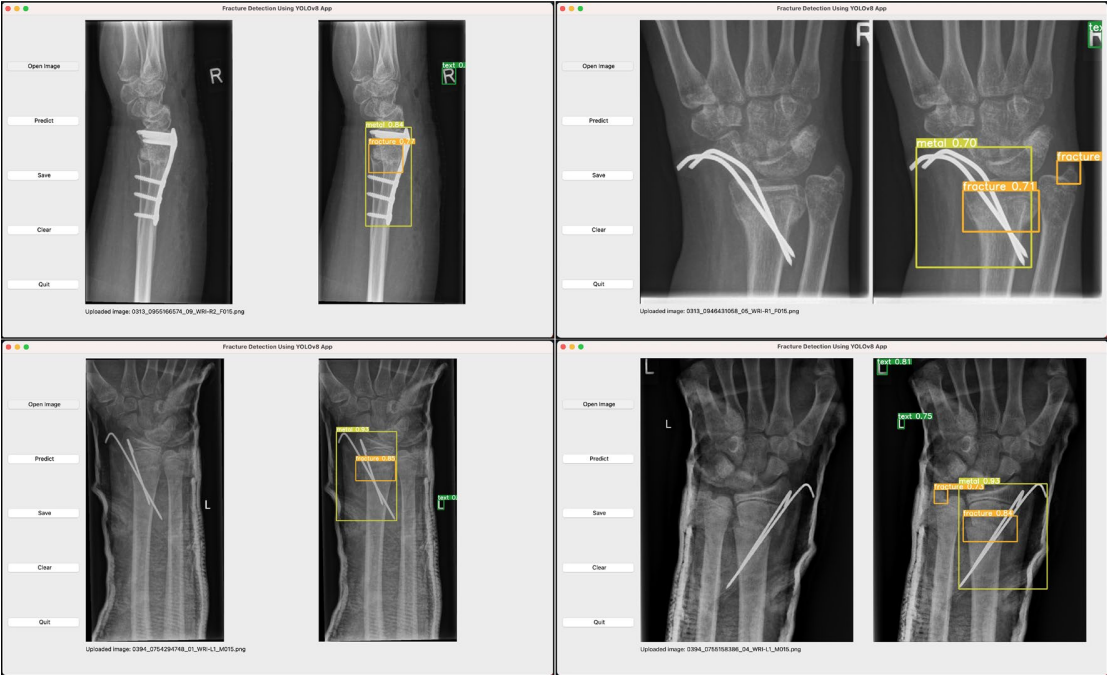
\includegraphics[width=0.5\textwidth]{images/FractureImple.png} 
  \caption{Example of using the application “Fracture Detection with YOLOv8 Application” on macOS
operating system. \cite{ju2023fracture}}
  \label{fig:Fracture example}
\end{figure}


\subsection{Algorithmic Improvements}
Next is looking at YOLOv8's algorithmic features and advancements over previous models. Like the switch to a different module for better object detection, this shows why YOLOv8  accurately identifies objects in images and videos.

\subsubsection{Different Module for Better Object Detection}
YOLOv8 moved from an anchor-based to an anchor-free detection module\cite{yolov8mmyolo2023}.This simplified how the model predicts bounding boxes and enhances its detection capabilities.

Anchor-based Detection \cite{MathWorksAnchorBoxes} :
Anchor-based detectors guess where objects might be by using pre-set shapes called anchors that are tiled across the image. It changes these shapes to fit the objects it come across.

There are two types: one-stage (fast) and two-stage (much more accurate).

Anchor-free detection \cite{LearnOpenCVCenterNet} :
Pre-set shapes are not used in anchor-free detectors. Instead, it detects objects in two ways:

Key point-based: This way locates important points such as corners or centers and uses them to determine the location of the entire object. It is more complicated, but it is a new look at object shapes.

Center-based: This way focuses on the center of an object and then calculates its size from there. It's similar to anchor-based but uses centers instead of pre-set shapes to create it.

The main difference is that anchor-free detectors do not use pre-set shapes making them simpler. 

\subsection{Reducing False Positives}
Getting the final results in object detection isn't just about finding objects, it also finding those objects accurately. YOLOv8 does this through an efficient step known as post-processing, and one of its key techniques is called Non-Maximum Suppression (NMS).

NMS plays a critical role in eliminating multiple detections of the same object. Which is a main source of false positives.

NMS\cite{NMS_Samb.k} works by ranking all the detections based on there confidence scores showing there likelihood of being a correct detection. It keeps the highest detection score based on the predefined overlap of the bounding box threshold. This process helps in resolving cases where multiple bounding boxes are detected around the same object where the false positive could be. The Effectiveness is a balancing act depending on the threshold as a strict threshold would miss on objects that are closely places, whilst a lenient threshold could keep redundant detections. By tuning this, YOLOv8 ensures that the confidence of the detections is maintained, making the output reliable and accurate.There is also now a better algorithm called 'soft-nms'\cite{bodla2017soft} which improves on accuracy.

\begin{figure}[ht]
\centering
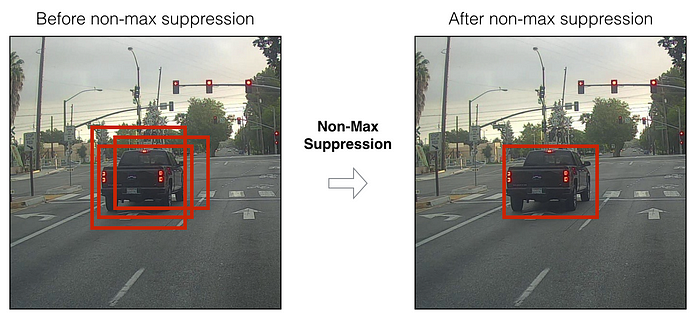
\includegraphics[width=0.5\textwidth]{images/NMS_Before_After.png}
\caption{Before and after non-maximum suppression \cite{NMS_Samb.k}.}
\label{fig:nms}
\end{figure}

A gap is seen in the data that impacts non-maximum suppression (NMS) on the accuracy of YOLOv8. With extensive searches across academic databases, journals, and conference proceedings. No metrics are found that compare the performance of YOLOv8 with and without the implementation of NMS. This shows the need for studies to show the use of NMS in enhancing the accuracy of advanced object detection models such as YOLOv8.

\section{Comparative Analysis of Object Detection Models}
In this section, three major object detection models are compared: Single-Shot Detection (SSD), You Only Look Once (YOLO), and Faster Region-Based Convolutional Neural Networks (FRCNN). The comparison is on a study\cite{Srivastava2021} on these models using the Microsoft COCO dataset\cite{cocodataset}. Focusing on average precision across the various Intersection over Union (IoU) thresholds and object sizes.

\subsection{Performance Metrics:}
This evaluation focuses on average precision\cite{kili_technology_map}. This is a measure that combines recall (how many actual positives were identified) and precision (how many identified positives were actually positive) across different IoU thresholds. The IoU thresholds help to know how well the models predicted bounding boxes match the ground truth. This analysis also considers object sizes (small, medium, and large) to see each model's effectiveness in detecting objects of different dimensions.

\subsection{YOLOv8 vs. R-CNN vs SSD}

\begin{table}[h]
\centering
\caption{Comparative Performance of Object Detection Models\cite{Srivastava2021}}
\label{tab:object_detection_models}
\resizebox{0.5\textwidth}{!}{%
\begin{tabular}{|l|c|c|c|c|}
\hline
Model & Small Objects & Medium Objects & Large Objects & Overall Precision \\ \hline
SSD   & 0.059         & 0.264          & 0.414         & 0.247             \\ \hline
YOLO  & 0.152         & 0.359          & 0.496         & 0.337             \\ \hline
FRCNN & 0.331         & 0.586          & 0.846         & 0.716             \\ \hline
\end{tabular}%
}
\end{table}


Using the data from above the performance is seen as per below:

FRCNN gives better average precision across all object sizes. Particularly in detecting large objects. It is a complex architecture to detect detailed features. But, the complex structure could lead to slower processing speeds that makes it less suitable for real-time applications.

YOLO is a balance between precision and speed. It performs better than SSD, especially in detecting medium and large objects. YOLO's design brings speed and efficiency which makes it perfect for real-time detection use cases, considering some trade-offs in precision compared to FRCNN.

SSD shows the lowest precision among the three models. As it is designed for speed, this comes at the cost of accuracy, especially in detecting smaller objects. SSD's architecture favors quicker detection times which may be more suited for applications where speed is more critical than high precision.


\section{Challenges and Limitations in Current Research}
\subsection{Addressing Complex Environments}
Current research on object detection faces challenges in dealing with complex environments, such as different lighting conditions, occlusions, and dynamic backgrounds\cite{article_limitations}. The need for object detection models to accurately identify objects is critical such as real world applications like autonomous driving and public safety surveillance. Continuous improvements are needed to enhance algorithms to adapt to these environmental factors.

\subsection{Ethical and Privacy Concerns}
Object detection applications collecting and analyzing data on individuals in public is a big privacy concern. Data like movements, interactions, personal attributes. This can be used for surveillance, profiling and targeted advertising. "Computer Vision applications retrieve information about individuals from visual data that is either pre-existing footage or gathered in real-time,".\cite{waelen2023ethics} This raises a concern about privacy violations and the potential misuse of personal information.

\section{Future Directions in Object Detection}
\subsection{Emerging Trends and Technologies}
As object detection models often need a lot of computing power to work quickly. Specialized hardware is in development that can speed up the process. such as field-programmable gate arrays (FPGAs)\cite{zeng2022fpga} to make object detection models more efficient. This makes them particularly for handling the real-time processing demands of complex object detection models like YOLOv8.

\begin{table}[ht]
\centering
\caption{Performance Comparison of Different Hardware Platforms \cite{li2022fpga}}
\label{table:hardware_comparison}
\resizebox{0.5\textwidth}{!}{%
\begin{tabular}{|l|c|c|c|}
\hline
\textbf{Platform} & \textbf{Intel Core i7 (CPU)} & \textbf{GeForce 1080ti (GPU)} & \textbf{Zynq-7000 (FPGA)} \\ \hline
Development Language & C & C & HLS \\ \hline
mAP & 82.60\% & 82.40\% & 80.60\% \\ \hline
Data Precision & Float & Float & Int8 \\ \hline
Power Consumption (W) & 122 & 249 & 2.6 \\ \hline
\end{tabular}%
}
\end{table}

PGA-based YOLO neural network accelerator\cite{li2022fpga} shows remarkable power efficiency with low power consumption. This FPGA in particular demonstrate significantly lower power usage (2.6W) compared to CPUs and GPUs. This optimization leaves much more room for additional processing tasks without affecting the performance accuracy of 80.6\% mAP. Also this FPGA accelerator shows a computing power of 27.1 GOP/s and efficient data processing which is a key metrics for real-time object detection applications.

\section{Conclusion}
This literature review aimed to provide a review of the evolution, current and the future of object detection. Focusing on the advancements made by YOLOv8. Throughout this review, a few of the technologies and methodologies have been reviewed from early object detection techniques to the developments in deep learning and neural networks. YOLOv8 with its single-pass approach and efficient algorithmic improvements, which represents a breakthrough in creating improved accuracy and speed over its predecessors.
\subsection{Summary of Key Findings}
The findings of this review show the critical role that object detection technology has. Especially in particular models like YOLOv8 in applications including medical diagnostics, public safety, and autonomous driving. Advances in accuracy and speed with the ability to process in complex environments. This shows a great step forward in using these technologies in applications. This review also highlighted existing gaps and limitations in the context of complex environments and ethical concerns related to privacy and data use.

\subsection{Implications for Future Research and Development}
A significant direction is the exploration of specialized hardware like FPGAs to enhance the efficiency of object detection models. There is a clear need for more research into the ethical and privacy aspects of object detection technology as it becomes seen more in everyday life and a need for implicit performance comparison in Non-Maximum Suppression (NMS) and how much it improves accuracy by. 

% references section
\printbibliography

\end{document}